\documentclass[]{article}
\usepackage{lmodern}
\usepackage{amssymb,amsmath}
\usepackage{ifxetex,ifluatex}
\usepackage{fixltx2e} % provides \textsubscript
\ifnum 0\ifxetex 1\fi\ifluatex 1\fi=0 % if pdftex
  \usepackage[T1]{fontenc}
  \usepackage[utf8]{inputenc}
\else % if luatex or xelatex
  \ifxetex
    \usepackage{mathspec}
  \else
    \usepackage{fontspec}
  \fi
  \defaultfontfeatures{Ligatures=TeX,Scale=MatchLowercase}
\fi
% use upquote if available, for straight quotes in verbatim environments
\IfFileExists{upquote.sty}{\usepackage{upquote}}{}
% use microtype if available
\IfFileExists{microtype.sty}{%
\usepackage{microtype}
\UseMicrotypeSet[protrusion]{basicmath} % disable protrusion for tt fonts
}{}
\usepackage[margin=1in]{geometry}
\usepackage{hyperref}
\hypersetup{unicode=true,
            pdftitle={Lab 6: Airport Data Science},
            pdfauthor={R-Kelly},
            pdfborder={0 0 0},
            breaklinks=true}
\urlstyle{same}  % don't use monospace font for urls
\usepackage{color}
\usepackage{fancyvrb}
\newcommand{\VerbBar}{|}
\newcommand{\VERB}{\Verb[commandchars=\\\{\}]}
\DefineVerbatimEnvironment{Highlighting}{Verbatim}{commandchars=\\\{\}}
% Add ',fontsize=\small' for more characters per line
\usepackage{framed}
\definecolor{shadecolor}{RGB}{248,248,248}
\newenvironment{Shaded}{\begin{snugshade}}{\end{snugshade}}
\newcommand{\KeywordTok}[1]{\textcolor[rgb]{0.13,0.29,0.53}{\textbf{#1}}}
\newcommand{\DataTypeTok}[1]{\textcolor[rgb]{0.13,0.29,0.53}{#1}}
\newcommand{\DecValTok}[1]{\textcolor[rgb]{0.00,0.00,0.81}{#1}}
\newcommand{\BaseNTok}[1]{\textcolor[rgb]{0.00,0.00,0.81}{#1}}
\newcommand{\FloatTok}[1]{\textcolor[rgb]{0.00,0.00,0.81}{#1}}
\newcommand{\ConstantTok}[1]{\textcolor[rgb]{0.00,0.00,0.00}{#1}}
\newcommand{\CharTok}[1]{\textcolor[rgb]{0.31,0.60,0.02}{#1}}
\newcommand{\SpecialCharTok}[1]{\textcolor[rgb]{0.00,0.00,0.00}{#1}}
\newcommand{\StringTok}[1]{\textcolor[rgb]{0.31,0.60,0.02}{#1}}
\newcommand{\VerbatimStringTok}[1]{\textcolor[rgb]{0.31,0.60,0.02}{#1}}
\newcommand{\SpecialStringTok}[1]{\textcolor[rgb]{0.31,0.60,0.02}{#1}}
\newcommand{\ImportTok}[1]{#1}
\newcommand{\CommentTok}[1]{\textcolor[rgb]{0.56,0.35,0.01}{\textit{#1}}}
\newcommand{\DocumentationTok}[1]{\textcolor[rgb]{0.56,0.35,0.01}{\textbf{\textit{#1}}}}
\newcommand{\AnnotationTok}[1]{\textcolor[rgb]{0.56,0.35,0.01}{\textbf{\textit{#1}}}}
\newcommand{\CommentVarTok}[1]{\textcolor[rgb]{0.56,0.35,0.01}{\textbf{\textit{#1}}}}
\newcommand{\OtherTok}[1]{\textcolor[rgb]{0.56,0.35,0.01}{#1}}
\newcommand{\FunctionTok}[1]{\textcolor[rgb]{0.00,0.00,0.00}{#1}}
\newcommand{\VariableTok}[1]{\textcolor[rgb]{0.00,0.00,0.00}{#1}}
\newcommand{\ControlFlowTok}[1]{\textcolor[rgb]{0.13,0.29,0.53}{\textbf{#1}}}
\newcommand{\OperatorTok}[1]{\textcolor[rgb]{0.81,0.36,0.00}{\textbf{#1}}}
\newcommand{\BuiltInTok}[1]{#1}
\newcommand{\ExtensionTok}[1]{#1}
\newcommand{\PreprocessorTok}[1]{\textcolor[rgb]{0.56,0.35,0.01}{\textit{#1}}}
\newcommand{\AttributeTok}[1]{\textcolor[rgb]{0.77,0.63,0.00}{#1}}
\newcommand{\RegionMarkerTok}[1]{#1}
\newcommand{\InformationTok}[1]{\textcolor[rgb]{0.56,0.35,0.01}{\textbf{\textit{#1}}}}
\newcommand{\WarningTok}[1]{\textcolor[rgb]{0.56,0.35,0.01}{\textbf{\textit{#1}}}}
\newcommand{\AlertTok}[1]{\textcolor[rgb]{0.94,0.16,0.16}{#1}}
\newcommand{\ErrorTok}[1]{\textcolor[rgb]{0.64,0.00,0.00}{\textbf{#1}}}
\newcommand{\NormalTok}[1]{#1}
\usepackage{longtable,booktabs}
\usepackage{graphicx,grffile}
\makeatletter
\def\maxwidth{\ifdim\Gin@nat@width>\linewidth\linewidth\else\Gin@nat@width\fi}
\def\maxheight{\ifdim\Gin@nat@height>\textheight\textheight\else\Gin@nat@height\fi}
\makeatother
% Scale images if necessary, so that they will not overflow the page
% margins by default, and it is still possible to overwrite the defaults
% using explicit options in \includegraphics[width, height, ...]{}
\setkeys{Gin}{width=\maxwidth,height=\maxheight,keepaspectratio}
\IfFileExists{parskip.sty}{%
\usepackage{parskip}
}{% else
\setlength{\parindent}{0pt}
\setlength{\parskip}{6pt plus 2pt minus 1pt}
}
\setlength{\emergencystretch}{3em}  % prevent overfull lines
\providecommand{\tightlist}{%
  \setlength{\itemsep}{0pt}\setlength{\parskip}{0pt}}
\setcounter{secnumdepth}{0}
% Redefines (sub)paragraphs to behave more like sections
\ifx\paragraph\undefined\else
\let\oldparagraph\paragraph
\renewcommand{\paragraph}[1]{\oldparagraph{#1}\mbox{}}
\fi
\ifx\subparagraph\undefined\else
\let\oldsubparagraph\subparagraph
\renewcommand{\subparagraph}[1]{\oldsubparagraph{#1}\mbox{}}
\fi

%%% Use protect on footnotes to avoid problems with footnotes in titles
\let\rmarkdownfootnote\footnote%
\def\footnote{\protect\rmarkdownfootnote}

%%% Change title format to be more compact
\usepackage{titling}

% Create subtitle command for use in maketitle
\newcommand{\subtitle}[1]{
  \posttitle{
    \begin{center}\large#1\end{center}
    }
}

\setlength{\droptitle}{-2em}

  \title{Lab 6: Airport Data Science}
    \pretitle{\vspace{\droptitle}\centering\huge}
  \posttitle{\par}
    \author{R-Kelly}
    \preauthor{\centering\large\emph}
  \postauthor{\par}
      \predate{\centering\large\emph}
  \postdate{\par}
    \date{2019-02-19}


\begin{document}
\maketitle

\section{Team Section}\label{team-section}

\subsection{Main Questions:}\label{main-questions}

\paragraph{What are the most likely factors to delay flights arriving in
Denver?}\label{what-are-the-most-likely-factors-to-delay-flights-arriving-in-denver}

It is interesting to note that the probability of a Late Aircraft Delay
occuring given that there is a arrival delay, is higher when looking at
the number of minutes produced by each delay versus the number of actual
delays. With that being said, Late Aircraft Delays, Carrier Delays, and
NAS Delays are still the most likely factor to delay flights arriving to
Denver.

\paragraph{What variables, if any, have no predictable effect on arrival
delays?}\label{what-variables-if-any-have-no-predictable-effect-on-arrival-delays}

As seen in Peter's individual plot, we can conclude that the average air
speed does not have a predictable effect on arrival delays. It is also
interesting to note that weather delays and security delays are the
least likely to be a factor for a delayed flight arriving to Denver.

\subsection{Team Plot:}\label{team-plot}

\begin{Shaded}
\begin{Highlighting}[]
\NormalTok{landed<-}\StringTok{ }\NormalTok{COflights }\OperatorTok\StringTok{ }\KeywordTok{filter}\NormalTok{(ORIGIN }\OperatorTok{==}\StringTok{ "DEN"}\NormalTok{, CANCELLED}\OperatorTok{==}\DecValTok{0}\NormalTok{)}

\NormalTok{late<-landed }\OperatorTok\StringTok{ }\KeywordTok{filter}\NormalTok{(ARR_DELAY}\OperatorTok{>=}\DecValTok{15}\NormalTok{) }\OperatorTok\StringTok{ }\KeywordTok{mutate}\NormalTok{(}\DataTypeTok{DELAY=} \KeywordTok{ifelse}\NormalTok{(WEATHER_DELAY }\OperatorTok{!=}\StringTok{ }\DecValTok{0}\NormalTok{,}\DecValTok{1}\NormalTok{,}\DecValTok{0}\NormalTok{) }\OperatorTok{+}\StringTok{ }\KeywordTok{ifelse}\NormalTok{(NAS_DELAY }\OperatorTok{!=}\StringTok{ }\DecValTok{0}\NormalTok{,}\DecValTok{1}\NormalTok{,}\DecValTok{0}\NormalTok{) }\OperatorTok{+}\StringTok{ }\KeywordTok{ifelse}\NormalTok{(SECURITY_DELAY }\OperatorTok{!=}\StringTok{ }\DecValTok{0}\NormalTok{,}\DecValTok{1}\NormalTok{,}\DecValTok{0}\NormalTok{) }\OperatorTok{+}\StringTok{ }\KeywordTok{ifelse}\NormalTok{(CARRIER_DELAY }\OperatorTok{!=}\StringTok{ }\DecValTok{0}\NormalTok{,}\DecValTok{1}\NormalTok{,}\DecValTok{0}\NormalTok{) }\OperatorTok{+}\StringTok{ }\KeywordTok{ifelse}\NormalTok{(LATE_AIRCRAFT_DELAY }\OperatorTok{!=}\StringTok{ }\DecValTok{0}\NormalTok{,}\DecValTok{1}\NormalTok{,}\DecValTok{0}\NormalTok{)) }

\NormalTok{delaytype <-}\StringTok{ }\KeywordTok{c}\NormalTok{(}\StringTok{"Carrier Delay"}\NormalTok{, }\StringTok{"Weather Delay"}\NormalTok{, }\StringTok{"NAS Delay"}\NormalTok{, }\StringTok{"Security Delay"}\NormalTok{, }\StringTok{"Late Aircraft Delay"}\NormalTok{)}

\NormalTok{total_time_delayed <-}\StringTok{ }\KeywordTok{c}\NormalTok{(}\KeywordTok{summarise}\NormalTok{(late, }\KeywordTok{sum}\NormalTok{(CARRIER_DELAY)),}\KeywordTok{summarise}\NormalTok{(late, }\KeywordTok{sum}\NormalTok{(WEATHER_DELAY)),}\KeywordTok{summarise}\NormalTok{(late, }\KeywordTok{sum}\NormalTok{(NAS_DELAY)),}\KeywordTok{summarise}\NormalTok{(late, }\KeywordTok{sum}\NormalTok{(SECURITY_DELAY)),}\KeywordTok{summarise}\NormalTok{(late, }\KeywordTok{sum}\NormalTok{(LATE_AIRCRAFT_DELAY)) )}
\NormalTok{delay_data <-}\StringTok{ }\KeywordTok{data.frame}\NormalTok{(delaytype, total_time_delayed)}
\KeywordTok{ggplot}\NormalTok{(delay_data)}\OperatorTok{+}\KeywordTok{geom_col}\NormalTok{(}\DataTypeTok{mapping =} \KeywordTok{aes}\NormalTok{(}\DataTypeTok{x=}\NormalTok{delaytype, }\DataTypeTok{y=}\NormalTok{total_time_delayed), }\DataTypeTok{fill =} \StringTok{'light pink'}\NormalTok{) }\OperatorTok{+}\StringTok{ }\KeywordTok{theme_minimal}\NormalTok{()}
\end{Highlighting}
\end{Shaded}

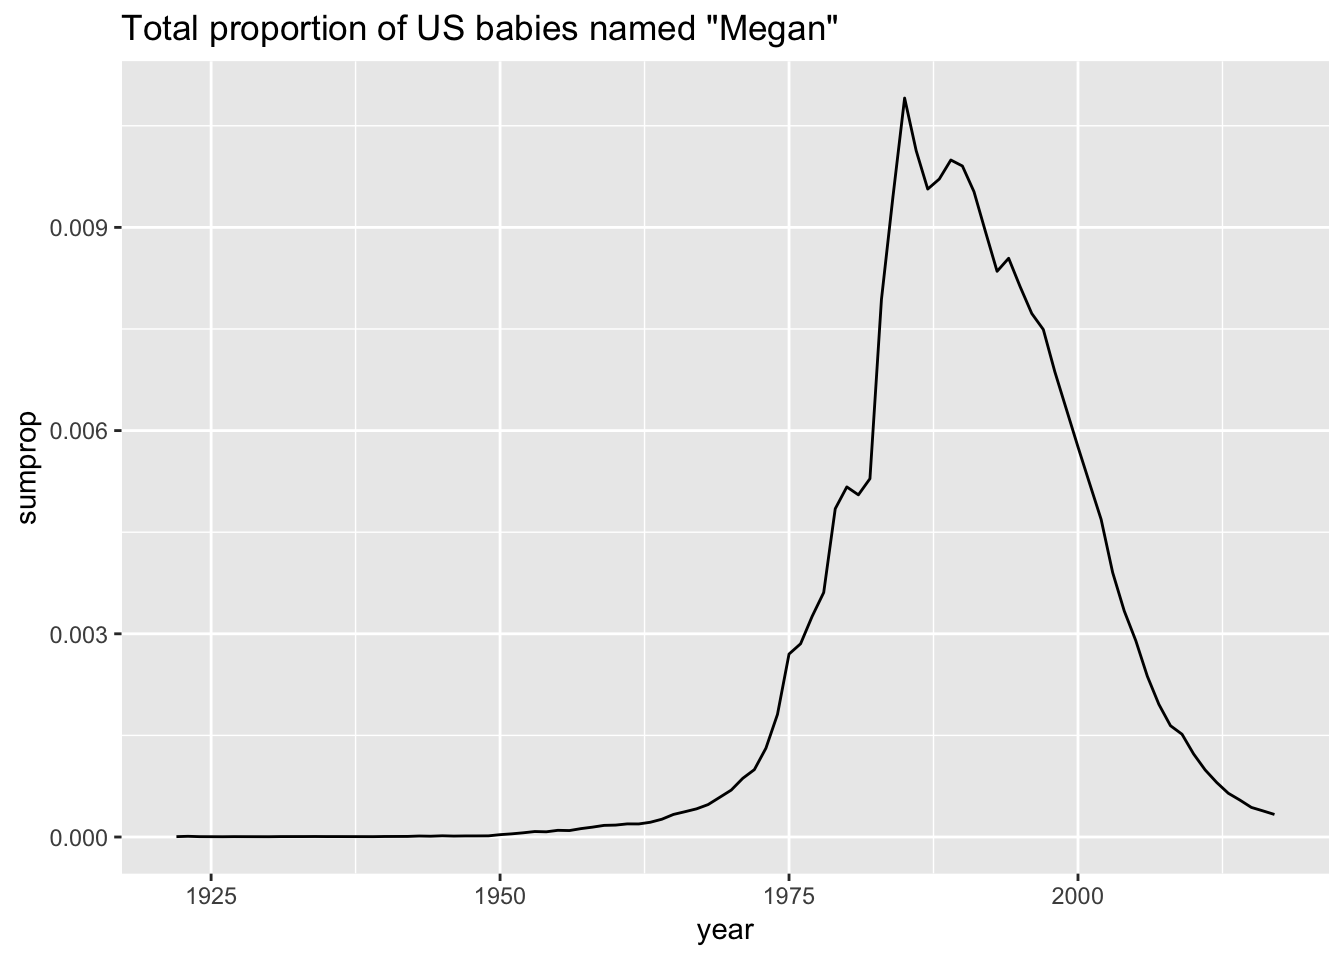
\includegraphics{Lab6_files/figure-latex/unnamed-chunk-2-1.pdf}

\subsection{Findings:}\label{findings}

\paragraph{Peter:}\label{peter}

I found that flight speed has almost no effect of the arrival delay of
flights, as the disrtibution of late flights matches that of flight
speed.

\paragraph{Ping:}\label{ping}

According to the plot I showed below, we can see that the month of the
year and different brands of the carriers do affect the delay of the
flights a little bit. We can see that May through August are the months
having the highest probability of a delayed flight. WN, UA, OO carriers
have the highest probability of having a delayed flight. So, all in all,
there is a higher chance of taking a delayed flight by WN, UA, and OO
carriers in May through August.

\subsection{Recomendation:}\label{recomendation}

\paragraph{Ping:}\label{ping-1}

When it comes to travelling, choose the months that are not that busy,
for example, months from Sep to April. Also, especially try to avoid
choosing WN, UA, OO carriers in busy months, because they have a higher
chance of being delayed.

\paragraph{Lauren:}\label{lauren}

I would recommend to the airport managers to focus on carrier delays
since this is the one variable which is most in the airline's control.
The managers should work on a more effective process in this area.

\subsubsection{Personal Section}\label{personal-section}

\paragraph{Peter}\label{peter-1}

This plot shows the relative distribution of flights delay times, and
their average air speed. This graph shows that there is almost no
correlation between arrival delay and airspeed of the flight.

\begin{Shaded}
\begin{Highlighting}[]
\NormalTok{Cflights <-}\StringTok{ }\KeywordTok{mutate}\NormalTok{(COflights, }\DataTypeTok{distAir =}\NormalTok{ DISTANCE}\OperatorTok{/}\NormalTok{AIR_TIME)}
\NormalTok{c <-}\StringTok{ }\KeywordTok{ggplot}\NormalTok{(}\DataTypeTok{data =}\NormalTok{ Cflights, }\DataTypeTok{mapping =} \KeywordTok{aes}\NormalTok{(}\DataTypeTok{x =}\NormalTok{ ARR_DELAY, }\DataTypeTok{y =}\NormalTok{ distAir)) }\OperatorTok{+}
\StringTok{   }\KeywordTok{geom_hex}\NormalTok{() }\OperatorTok{+}
\StringTok{   }\KeywordTok{geom_smooth}\NormalTok{()}
\KeywordTok{print}\NormalTok{(c)}
\end{Highlighting}
\end{Shaded}

\includegraphics{Lab6_files/figure-latex/unnamed-chunk-3-1.pdf}

\paragraph{Lauren}\label{lauren-1}

\begin{Shaded}
\begin{Highlighting}[]
\NormalTok{nlate<-}\StringTok{ }\KeywordTok{summarise}\NormalTok{(late, }\KeywordTok{sum}\NormalTok{(DELAY))}

\NormalTok{nweather<-landed }\OperatorTok\StringTok{ }\KeywordTok{filter}\NormalTok{(ARR_DELAY}\OperatorTok{>=}\DecValTok{15} \OperatorTok{&}\StringTok{ }\NormalTok{WEATHER_DELAY}\OperatorTok{>}\DecValTok{0}\NormalTok{) }\OperatorTok\StringTok{ }\KeywordTok{count}\NormalTok{()}
\NormalTok{pweather<-nweather}\OperatorTok{/}\NormalTok{nlate}

\NormalTok{ncarrier<-landed }\OperatorTok\StringTok{ }\KeywordTok{filter}\NormalTok{(ARR_DELAY}\OperatorTok{>=}\DecValTok{15} \OperatorTok{&}\StringTok{ }\NormalTok{CARRIER_DELAY}\OperatorTok{>}\DecValTok{0}\NormalTok{) }\OperatorTok\StringTok{ }\KeywordTok{count}\NormalTok{()}
\NormalTok{pcarrier<-ncarrier}\OperatorTok{/}\NormalTok{nlate}

\NormalTok{nnas<-landed }\OperatorTok\StringTok{ }\KeywordTok{filter}\NormalTok{(ARR_DELAY}\OperatorTok{>=}\DecValTok{15} \OperatorTok{&}\StringTok{ }\NormalTok{NAS_DELAY}\OperatorTok{>}\DecValTok{0}\NormalTok{) }\OperatorTok\StringTok{ }\KeywordTok{count}\NormalTok{()}
\NormalTok{pnas<-nnas}\OperatorTok{/}\NormalTok{nlate}

\NormalTok{nsecurity<-landed }\OperatorTok\StringTok{ }\KeywordTok{filter}\NormalTok{(ARR_DELAY}\OperatorTok{>=}\DecValTok{15} \OperatorTok{&}\StringTok{ }\NormalTok{SECURITY_DELAY}\OperatorTok{>}\DecValTok{0}\NormalTok{) }\OperatorTok\StringTok{ }\KeywordTok{count}\NormalTok{()}
\NormalTok{psecurity<-nsecurity}\OperatorTok{/}\NormalTok{nlate}

\NormalTok{nlateaircraft<-landed }\OperatorTok\StringTok{ }\KeywordTok{filter}\NormalTok{(ARR_DELAY}\OperatorTok{>=}\DecValTok{15} \OperatorTok{&}\StringTok{ }\NormalTok{LATE_AIRCRAFT_DELAY}\OperatorTok{>}\DecValTok{0}\NormalTok{) }\OperatorTok\StringTok{ }\KeywordTok{count}\NormalTok{()}
\NormalTok{plateaircraft<-nlateaircraft}\OperatorTok{/}\NormalTok{nlate}
\end{Highlighting}
\end{Shaded}

\begin{Shaded}
\begin{Highlighting}[]
\NormalTok{delaytype <-}\StringTok{ }\KeywordTok{c}\NormalTok{(}\StringTok{"Carrier Delay"}\NormalTok{, }\StringTok{"Weather Delay"}\NormalTok{, }\StringTok{"NAS Delay"}\NormalTok{, }\StringTok{"Security Delay"}\NormalTok{, }\StringTok{"Late Aircraft Delay"}\NormalTok{)}
\NormalTok{amount_of_delays <-}\StringTok{ }\KeywordTok{c}\NormalTok{(}\DecValTok{20997}\NormalTok{,}\DecValTok{1667}\NormalTok{,}\DecValTok{23199}\NormalTok{,}\DecValTok{38}\NormalTok{,}\DecValTok{21087}\NormalTok{ )}
\NormalTok{delay_data <-}\StringTok{ }\KeywordTok{data.frame}\NormalTok{(delaytype, amount_of_delays)}
\KeywordTok{ggplot}\NormalTok{(delay_data)}\OperatorTok{+}\KeywordTok{geom_col}\NormalTok{(}\DataTypeTok{mapping =} \KeywordTok{aes}\NormalTok{(}\DataTypeTok{x=}\NormalTok{delaytype, }\DataTypeTok{y=}\NormalTok{amount_of_delays)) }\OperatorTok{+}\StringTok{ }\KeywordTok{theme_dark}\NormalTok{()}
\end{Highlighting}
\end{Shaded}

\includegraphics{Lab6_files/figure-latex/unnamed-chunk-5-1.pdf}

From this representation of the data it is clear that the largest amount
of Arrival Delays occurs due to National Air System delays, with delays
due to Late Aircraft and Carrier Delays close behind. The proabilities
of each delay type occuring based on the number of delays (not the
delays in minutes) is as follows.

\begin{longtable}[]{@{}lllll@{}}
\toprule
Carrier Delay & Weather Delay & NAS Delay & Security Delay & Late
Aircraft Delay\tabularnewline
\midrule
\endhead
31.3\% & 2.49\% & 34.6\% & .0567\% & 31.5\%\tabularnewline
\bottomrule
\end{longtable}

\paragraph{Gregor}\label{gregor}

Probability of flight that has delayed taxi out is delayed with arrival
is:

\begin{verbatim}
##          n
## 1 10.08853
\end{verbatim}

Probability of flight that has delayed taxi in is delayed with arrival
is:

\begin{verbatim}
##          n
## 1 1.621614
\end{verbatim}

Creating vectors to contain names and values

\begin{Shaded}
\begin{Highlighting}[]
\NormalTok{x =}\StringTok{ }\KeywordTok{c}\NormalTok{(}\StringTok{"Probability of flights that had late taxi times on arrival being delayed"}\NormalTok{, }\StringTok{"Probability of flights that had late taxi times on departure being delayed"}\NormalTok{)}

\NormalTok{y =}\StringTok{ }\KeywordTok{c}\NormalTok{(num_late_taxi_in_delayed[}\DecValTok{1}\NormalTok{][}\DecValTok{1}\NormalTok{] }\OperatorTok{/}\StringTok{ }\KeywordTok{count}\NormalTok{(COflights) }\OperatorTok{*}\StringTok{ }\DecValTok{100}\NormalTok{, num_late_taxi_out_delayed[}\DecValTok{1}\NormalTok{][}\DecValTok{1}\NormalTok{] }\OperatorTok{/}\StringTok{ }\KeywordTok{count}\NormalTok{(COflights)}\OperatorTok{*}\DecValTok{100}\NormalTok{)}
\end{Highlighting}
\end{Shaded}

Creating Tibble

\begin{Shaded}
\begin{Highlighting}[]
\NormalTok{GraphData <-}\StringTok{ }\KeywordTok{tibble}\NormalTok{(x, y)}
\end{Highlighting}
\end{Shaded}

\begin{Shaded}
\begin{Highlighting}[]
\KeywordTok{ggplot}\NormalTok{(}\DataTypeTok{data =}\NormalTok{ GraphData, }\KeywordTok{aes}\NormalTok{(}\DataTypeTok{x =}\NormalTok{ x, }\DataTypeTok{y =}\NormalTok{ y)) }\OperatorTok{+}\StringTok{ }\KeywordTok{geom_bar}\NormalTok{(}\DataTypeTok{stat =} \StringTok{"identity"}\NormalTok{) }\OperatorTok{+}\StringTok{ }\KeywordTok{coord_flip}\NormalTok{() }\OperatorTok{+}\StringTok{ }\KeywordTok{ylab}\NormalTok{(}\StringTok{"Percentage"}\NormalTok{) }\OperatorTok{+}\StringTok{ }\KeywordTok{xlab}\NormalTok{(}\StringTok{"Type of taxi delay"}\NormalTok{)}
\end{Highlighting}
\end{Shaded}

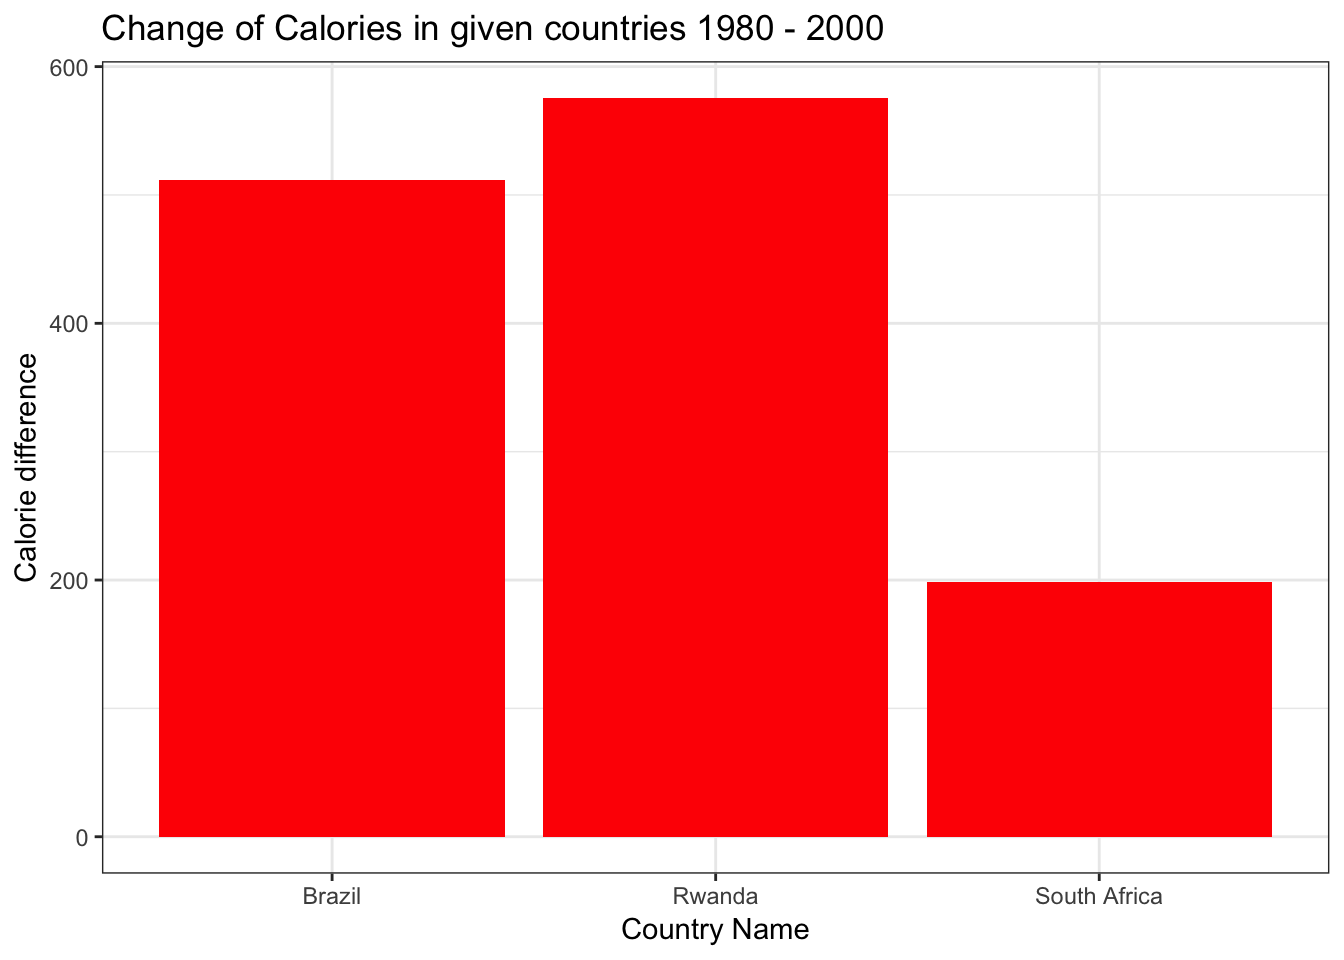
\includegraphics{Lab6_files/figure-latex/unnamed-chunk-11-1.pdf}

With these results, it is clear that taxing on DENs side doesn't affect
whether the flight is delayed. However, it is unknown whether the
arrival time is recorded before or after taxing. If it is recorded after
taxing, then this information is significant as it shows that DEN
airport is efficient in taxing, since there's a low chance that flights
that are delayed is due to late taxing. However, if the arrival time is
recorded before taxing, then this information is insignificant in
relation to identifying what DEN airport can do to adjust for preventing
delayed flights.

When flights that have a delayed taxi time leaving the origin airport to
DEN, there's about a 10\% chance that they will be delayed coming into
DEN. The airport could perhaps use this information as if they see a
flight has a taxi time of more than 15 minutes, than they can expect
that 10\% of the time it will be a delayed flight, which can be used to
inform people that are awaiting passsengers of that flight.

\paragraph{Sasha}\label{sasha}

\begin{Shaded}
\begin{Highlighting}[]
\NormalTok{ firstHalf <-}\StringTok{ }\KeywordTok{filter}\NormalTok{(COflights, DAY_OF_MONTH }\OperatorTok{<=}\StringTok{ }\DecValTok{15}\NormalTok{)}
\NormalTok{firstHalfDelayed <-}\StringTok{ }\KeywordTok{count}\NormalTok{(}\KeywordTok{filter}\NormalTok{(firstHalf, ARR_DELAY }\OperatorTok{>=}\StringTok{ }\DecValTok{15}\NormalTok{))}
\NormalTok{firstHalfDelayed[}\DecValTok{1}\NormalTok{][}\DecValTok{1}\NormalTok{] }\OperatorTok{/}\StringTok{ }\KeywordTok{count}\NormalTok{(COflights) }\OperatorTok{*}\StringTok{ }\DecValTok{100}
\end{Highlighting}
\end{Shaded}

\begin{verbatim}
##          n
## 1 8.752981
\end{verbatim}

\begin{Shaded}
\begin{Highlighting}[]
\NormalTok{secondHalf <-}\StringTok{ }\KeywordTok{filter}\NormalTok{(COflights, DAY_OF_MONTH }\OperatorTok{>}\DecValTok{15}\NormalTok{)}
\NormalTok{secondHalfDelayed <-}\StringTok{ }\KeywordTok{count}\NormalTok{(}\KeywordTok{filter}\NormalTok{(secondHalf, ARR_DELAY }\OperatorTok{>=}\StringTok{ }\DecValTok{15}\NormalTok{))}
\NormalTok{secondHalfDelayed[}\DecValTok{1}\NormalTok{][}\DecValTok{1}\NormalTok{] }\OperatorTok{/}\StringTok{ }\KeywordTok{count}\NormalTok{(COflights) }\OperatorTok{*}\StringTok{ }\DecValTok{100}
\end{Highlighting}
\end{Shaded}

\begin{verbatim}
##          n
## 1 8.483061
\end{verbatim}

\begin{Shaded}
\begin{Highlighting}[]
\KeywordTok{ggplot}\NormalTok{(}\DataTypeTok{data =}\NormalTok{ firstHalf) }\OperatorTok{+}\StringTok{ }
\StringTok{  }\KeywordTok{geom_bar}\NormalTok{(}\DataTypeTok{mapping =} \KeywordTok{aes}\NormalTok{(}\DataTypeTok{x =}\NormalTok{ ARR_DELAY))}\OperatorTok{+}\StringTok{ }\KeywordTok{xlim}\NormalTok{(}\DecValTok{0}\NormalTok{,}\DecValTok{60}\NormalTok{) }\OperatorTok{+}\StringTok{ }\KeywordTok{xlab}\NormalTok{( }\StringTok{"Arrival Delay"}\NormalTok{)}
\end{Highlighting}
\end{Shaded}

\begin{verbatim}
## Warning: Removed 162877 rows containing non-finite values (stat_count).
\end{verbatim}

\begin{verbatim}
## Warning: Removed 2 rows containing missing values (geom_bar).
\end{verbatim}

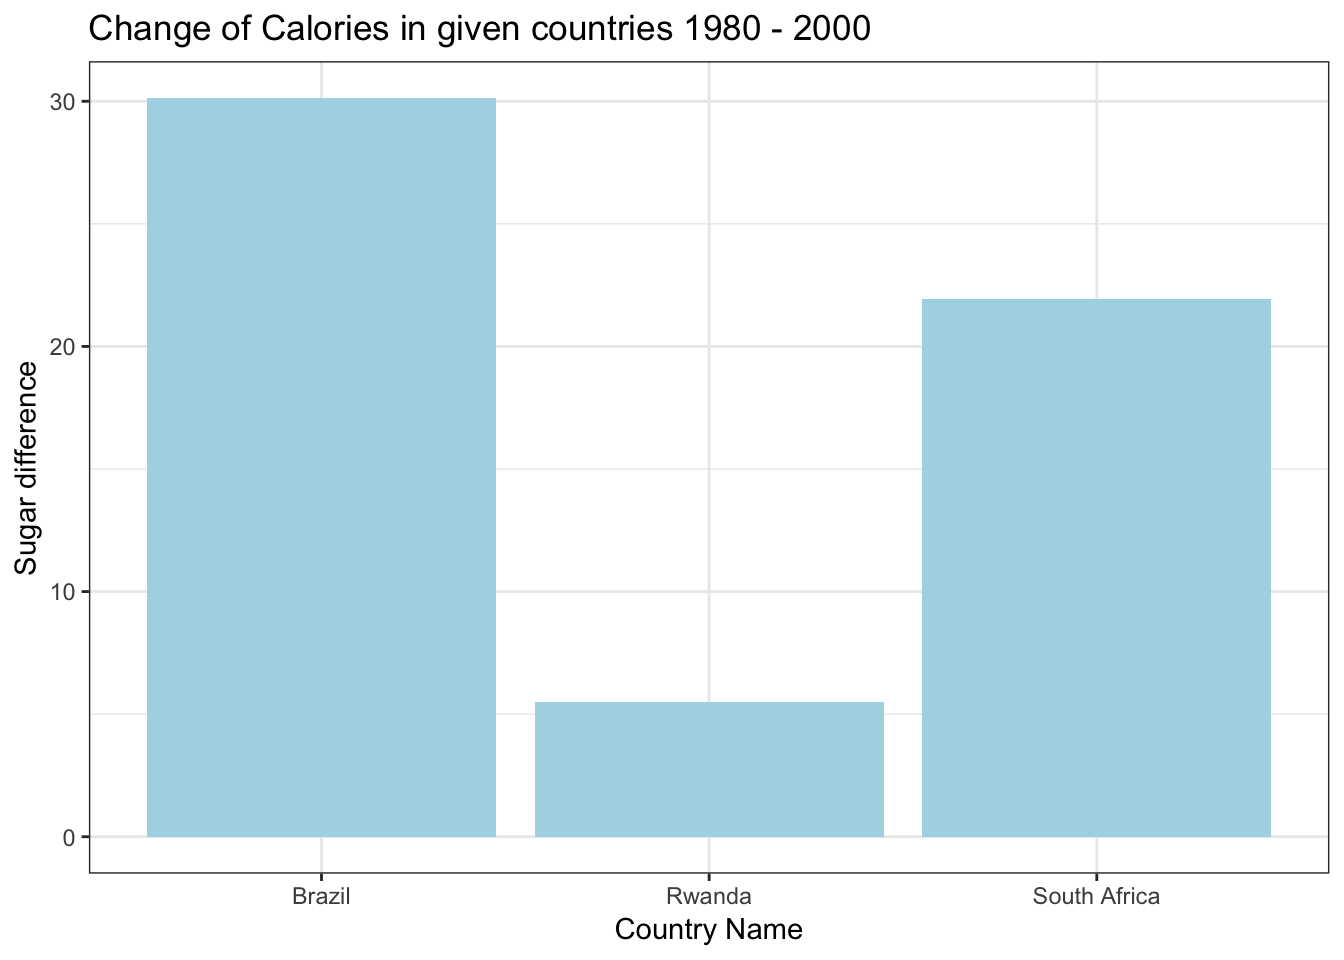
\includegraphics{Lab6_files/figure-latex/unnamed-chunk-13-1.pdf}

\begin{Shaded}
\begin{Highlighting}[]
\KeywordTok{ggplot}\NormalTok{(}\DataTypeTok{data =}\NormalTok{ secondHalf) }\OperatorTok{+}\StringTok{ }
\StringTok{  }\KeywordTok{geom_bar}\NormalTok{(}\DataTypeTok{mapping =} \KeywordTok{aes}\NormalTok{(}\DataTypeTok{x =}\NormalTok{ ARR_DELAY))}\OperatorTok{+}\StringTok{ }\KeywordTok{xlim}\NormalTok{(}\DecValTok{0}\NormalTok{,}\DecValTok{60}\NormalTok{) }\OperatorTok{+}\StringTok{ }\KeywordTok{xlab}\NormalTok{( }\StringTok{"Arrival Delay"}\NormalTok{)}
\end{Highlighting}
\end{Shaded}

\begin{verbatim}
## Warning: Removed 170796 rows containing non-finite values (stat_count).

## Warning: Removed 2 rows containing missing values (geom_bar).
\end{verbatim}

\includegraphics{Lab6_files/figure-latex/unnamed-chunk-13-2.pdf}

\paragraph{Ping}\label{ping-2}

I try to explore how can the month of the year and the brands of the
carriers affect the delay of the flight to Denver.

\begin{Shaded}
\begin{Highlighting}[]
\NormalTok{DenDelayed_Month_Carrier <-}\StringTok{ }\NormalTok{COflights }\OperatorTok\StringTok{ }\KeywordTok{filter}\NormalTok{(DEST }\OperatorTok{==}\StringTok{ "DEN"}\NormalTok{, ARR_DELAY }\OperatorTok{>=}\StringTok{ }\DecValTok{15}\NormalTok{) }\OperatorTok\StringTok{ }\KeywordTok{select}\NormalTok{(YEAR, MONTH, CARRIER, ARR_DELAY)}
\KeywordTok{ggplot}\NormalTok{(}\DataTypeTok{data =}\NormalTok{ DenDelayed_Month_Carrier) }\OperatorTok{+}\StringTok{ }\KeywordTok{geom_bar}\NormalTok{(}\DataTypeTok{mapping =} \KeywordTok{aes}\NormalTok{(}\DataTypeTok{x =}\NormalTok{ MONTH, }\DataTypeTok{fill =}\NormalTok{ CARRIER)) }\OperatorTok{+}\StringTok{ }\KeywordTok{xlim}\NormalTok{(}\DecValTok{0}\NormalTok{,}\DecValTok{13}\NormalTok{)}
\end{Highlighting}
\end{Shaded}

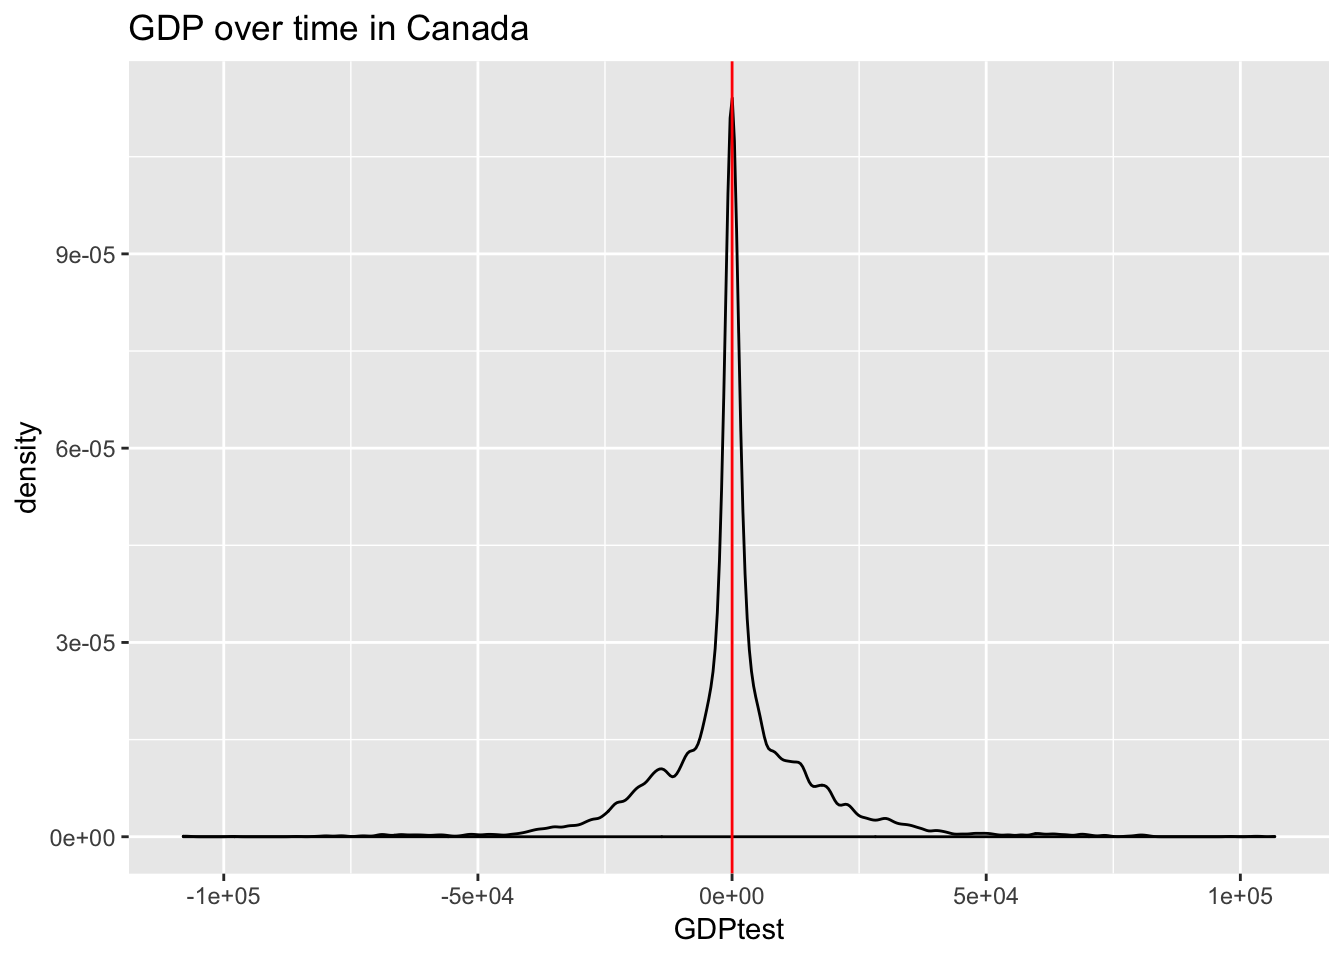
\includegraphics{Lab6_files/figure-latex/unnamed-chunk-14-1.pdf}

\begin{Shaded}
\begin{Highlighting}[]
\NormalTok{total_allMonths <-}\StringTok{ }\NormalTok{DenDelayed_Month_Carrier }\OperatorTok\StringTok{ }\KeywordTok{count}\NormalTok{()}
\NormalTok{highlyDelayedCount <-}\StringTok{ }\NormalTok{DenDelayed_Month_Carrier }\OperatorTok\StringTok{ }\KeywordTok{filter}\NormalTok{((MONTH }\OperatorTok\StringTok{ }\KeywordTok{c}\NormalTok{(}\DecValTok{5}\NormalTok{, }\DecValTok{8}\NormalTok{)))  }\OperatorTok\StringTok{ }\KeywordTok{count}\NormalTok{()}
\NormalTok{prob <-}\StringTok{ }\NormalTok{(highlyDelayedCount}\OperatorTok{/}\NormalTok{total_allMonths)}

\NormalTok{pro_may_aug_lowdelayed <-}\StringTok{ }\NormalTok{(DenDelayed_Month_Carrier }\OperatorTok\StringTok{ }\KeywordTok{filter}\NormalTok{(CARRIER }\OperatorTok\StringTok{ }\KeywordTok{c}\NormalTok{(}\StringTok{"DL"}\NormalTok{, }\StringTok{"AA"}\NormalTok{, }\StringTok{"VX"}\NormalTok{)) }\OperatorTok\StringTok{ }\KeywordTok{count}\NormalTok{()) }\OperatorTok{/}\StringTok{ }\NormalTok{total_allMonths}

\NormalTok{pro_may_aug_highdelayed <-}\StringTok{ }\NormalTok{(DenDelayed_Month_Carrier }\OperatorTok\StringTok{ }\KeywordTok{filter}\NormalTok{(CARRIER }\OperatorTok\StringTok{ }\KeywordTok{c}\NormalTok{(}\StringTok{"WN"}\NormalTok{, }\StringTok{"VA"}\NormalTok{, }\StringTok{"OO"}\NormalTok{)) }\OperatorTok\StringTok{ }\KeywordTok{count}\NormalTok{()) }\OperatorTok{/}\StringTok{ }\NormalTok{total_allMonths}
\end{Highlighting}
\end{Shaded}

We can see from the information above, that the probability of a delayed
flight in May through August is 20.58\%. In May through August, if you
take the flights of WN, UA, OO, there is a even higher chance of being
delayed(53.34\%), compaing to taking DL, AA, VX(11.16\%).

\subsection{What we did:}\label{what-we-did}

\subsubsection{Peter:}\label{peter-2}

I examined the relationship between average airspeed and arrival delay,
as well as helped with the formatting of the report and formulation of
our research questions.

\subsubsection{Lauren}\label{lauren-2}

I examined the probability of different delay types given that a flight
was delayed by calculating probabilities and representing the data in a
bar graph.

\subsubsection{Gregor}\label{gregor-1}

Examined the probability of flights that have delayed taxi times
delaying the actual arrival time of the flight

\subsubsection{Sasha:}\label{sasha-1}

I explored the probablity of arrival delay for flights that occur in the
first half of the month (until the 15th day) and then also the second
half of the month. According to the data, it is more probable that a
flight will have an arrival delay earlier in the month as opposed to
later.

\subsubsection{Ping:}\label{ping-3}

I explored the relationship between month, carriers and the delayed
flights. I also helped with the conclusion of the Team Findings.


\end{document}
